\chapter{GRÁFICOS DAS TENSÕES COM CLASSIFICAÇÃO - AMOSTRA 1}
\label{ap:graficos_a1}


\begin{figure}[H]
	\centering
	\caption{Gráfico para tensão V1 de fase média}
    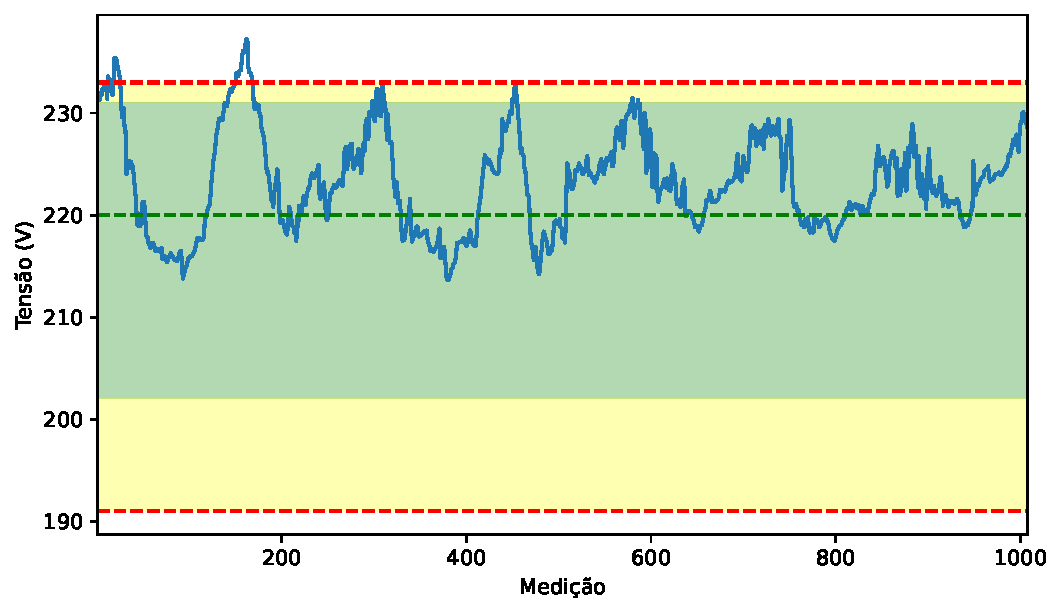
\includegraphics[width=16cm]{illustrations/figures/a1_V1_Avg.pdf}
	\fonte{Autoria própria.}
\end{figure}

\begin{figure}[H]
	\centering
	\caption{Gráfico para tensão V2 de fase média}
    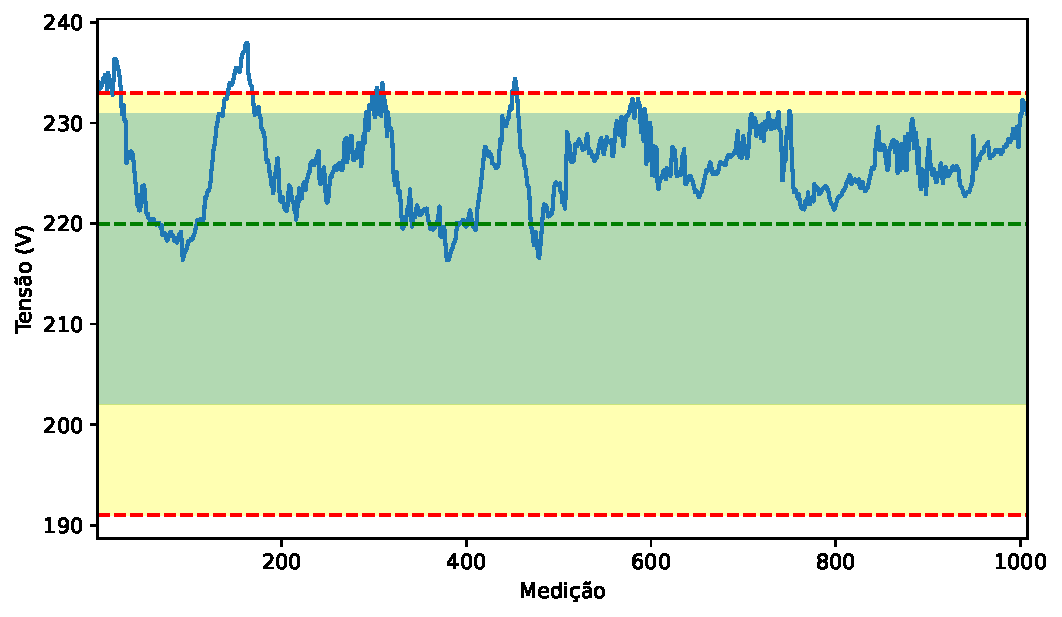
\includegraphics[width=16cm]{illustrations/figures/a1_V2_Avg.pdf}
	\fonte{Autoria própria.}
\end{figure}

\begin{figure}[H]
	\centering
	\caption{Gráfico para tensão V3 de fase média}
    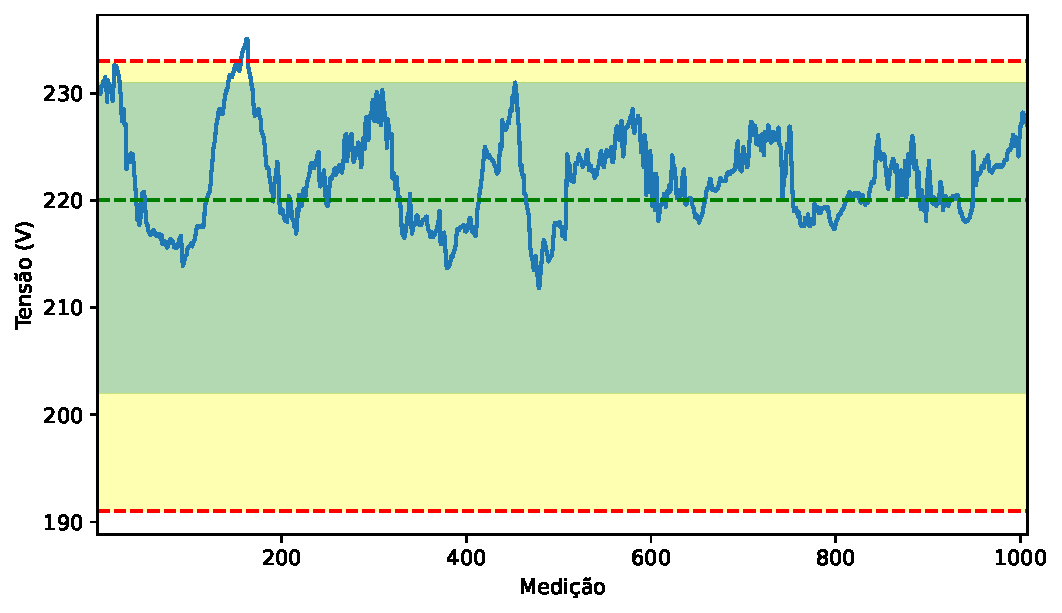
\includegraphics[width=16cm]{illustrations/figures/a1_V3_Avg.pdf}
	\fonte{Autoria própria.}
\end{figure}

\begin{figure}[H]
	\centering
	\caption{Gráfico para tensão V1 de fase máxima}
    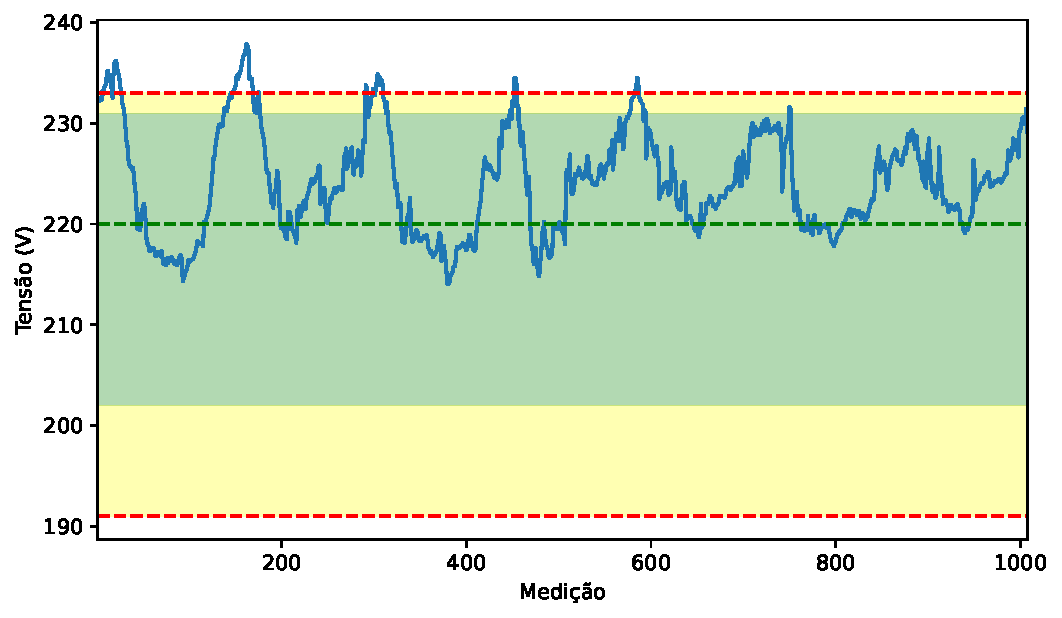
\includegraphics[width=16cm]{illustrations/figures/a1_V1_Max.pdf}
	\fonte{Autoria própria.}
\end{figure}

\begin{figure}[H]
	\centering
	\caption{Gráfico para tensão V2 de fase máxima}
    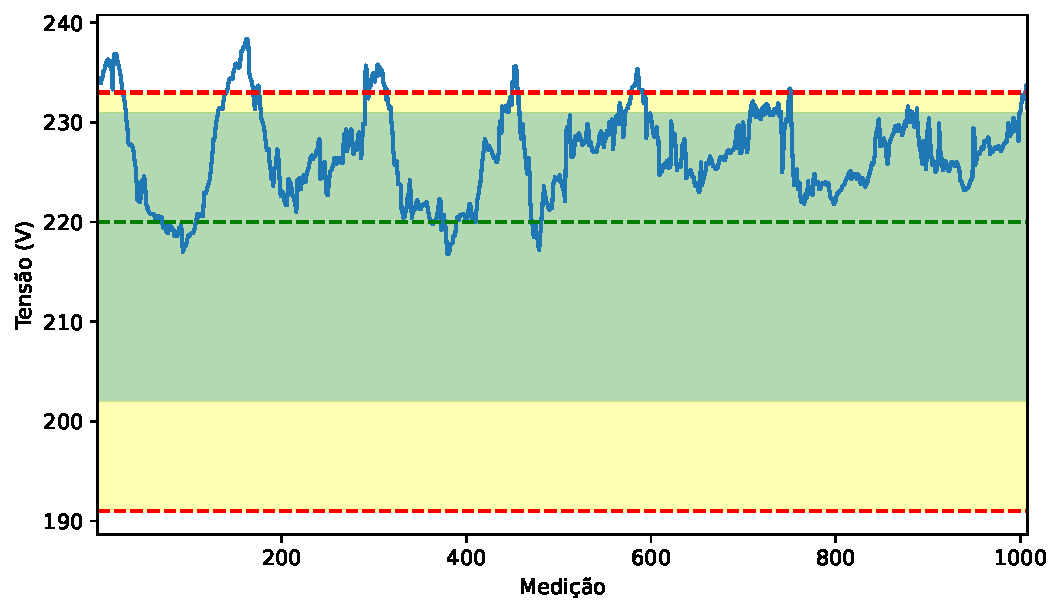
\includegraphics[width=16cm]{illustrations/figures/a1_V2_Max.pdf}
	\fonte{Autoria própria.}
\end{figure}

\begin{figure}[H]
	\centering
	\caption{Gráfico para tensão V3 de fase máxima}
    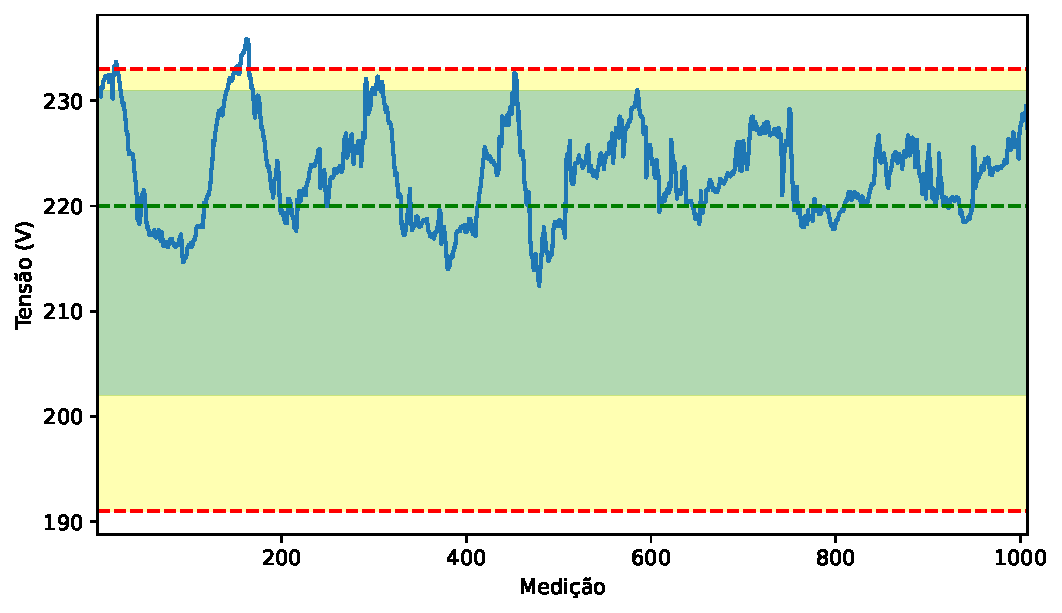
\includegraphics[width=16cm]{illustrations/figures/a1_V3_Max.pdf}
	\fonte{Autoria própria.}
\end{figure}

\begin{figure}[H]
	\centering
	\caption{Gráfico para tensão V1 de fase mínima}
    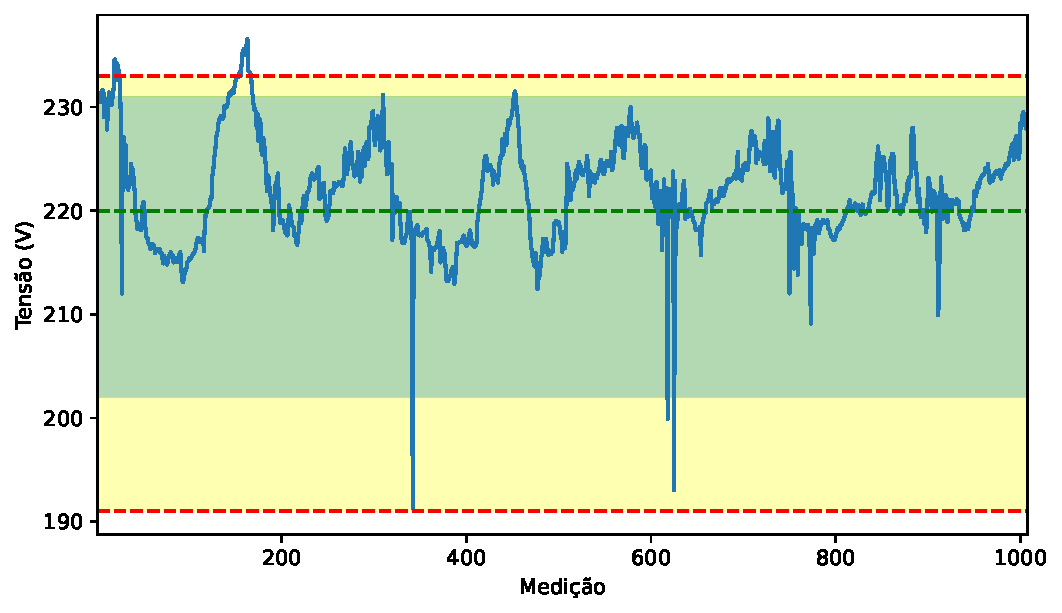
\includegraphics[width=16cm]{illustrations/figures/a1_V1_Min.pdf}
	\fonte{Autoria própria.}
\end{figure}

\begin{figure}[H]
	\centering
	\caption{Gráfico para tensão V2 de fase mínima}
    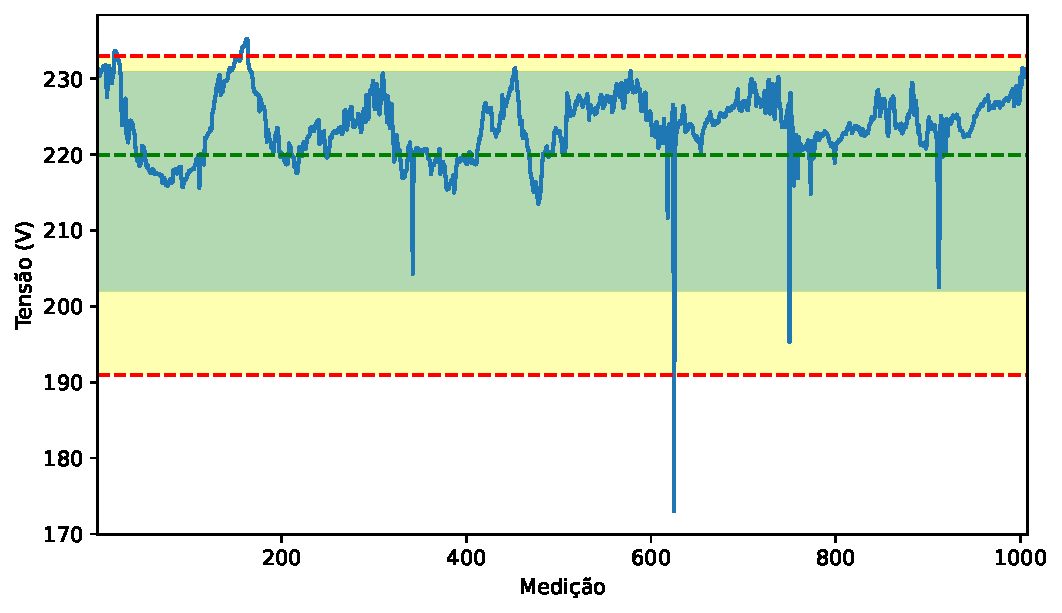
\includegraphics[width=16cm]{illustrations/figures/a1_V2_Min.pdf}
	\fonte{Autoria própria.}
\end{figure}

\begin{figure}[H]
	\centering
	\caption{Gráfico para tensão V3 de fase mínima}
    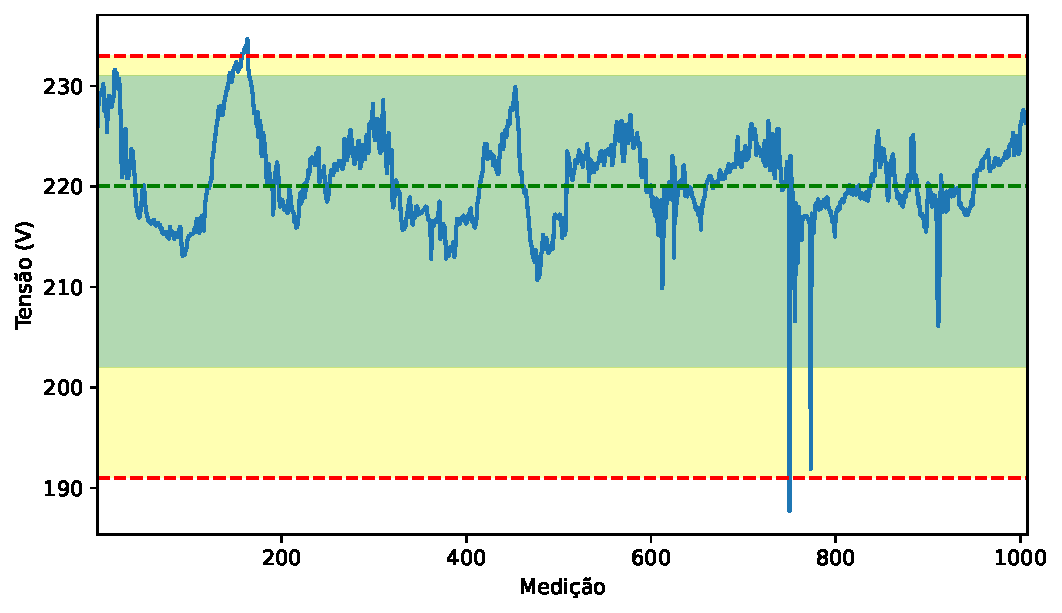
\includegraphics[width=16cm]{illustrations/figures/a1_V3_Min.pdf}
	\fonte{Autoria própria.}
\end{figure}

\begin{figure}[H]
	\centering
	\caption{Gráfico para tensão V12 de linha média}
    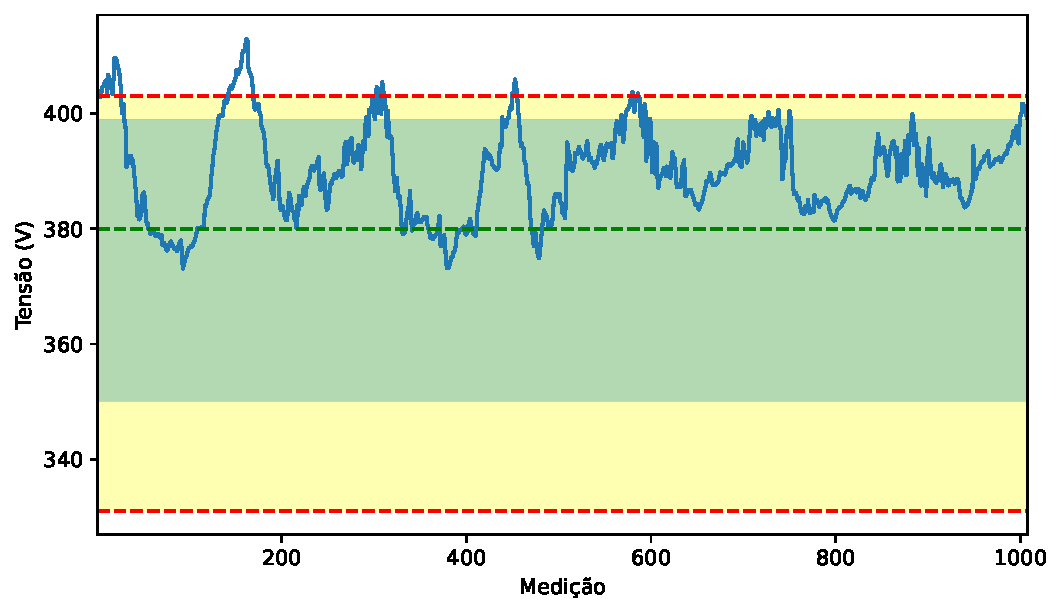
\includegraphics[width=16cm]{illustrations/figures/a1_V12_Avg.pdf}
	\fonte{Autoria própria.}
\end{figure}

\begin{figure}[H]
	\centering
	\caption{Gráfico para tensão V23 de linha média}
    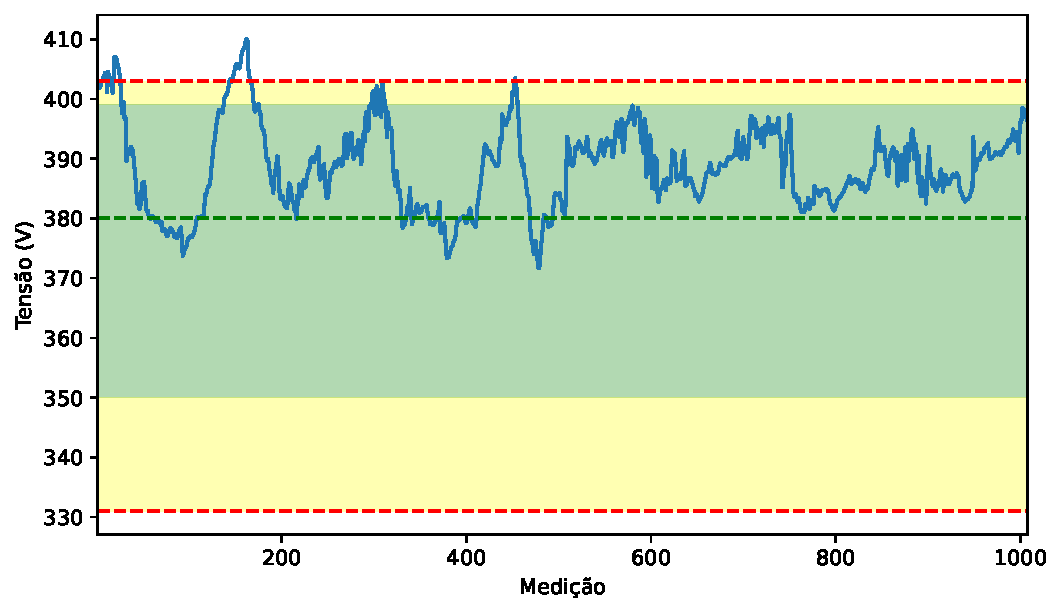
\includegraphics[width=16cm]{illustrations/figures/a1_V23_Avg.pdf}
	\fonte{Autoria própria.}
\end{figure}

\begin{figure}[H]
	\centering
	\caption{Gráfico para tensão V31 de linha média}
    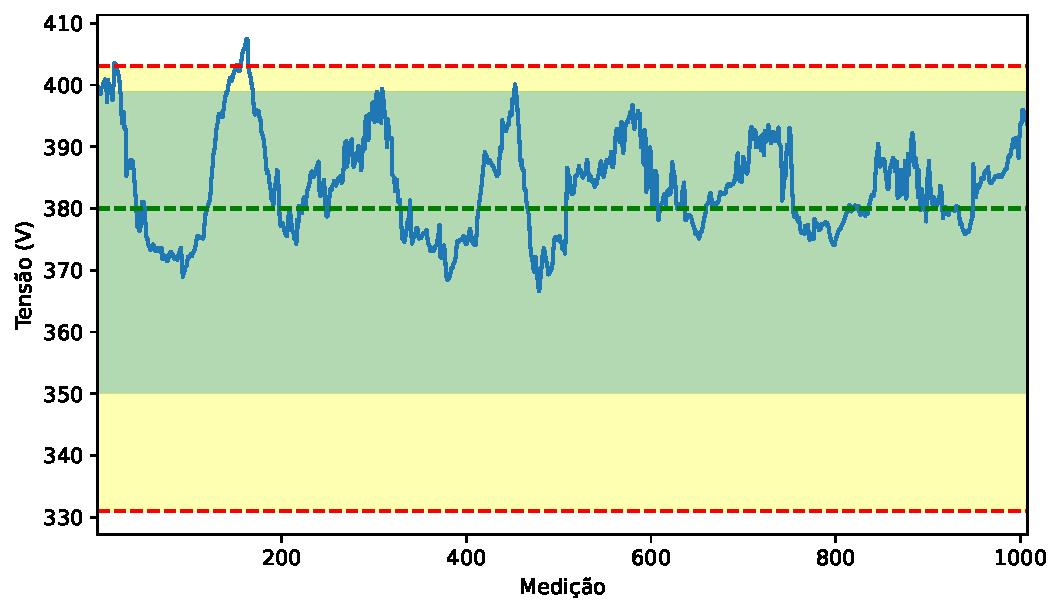
\includegraphics[width=16cm]{illustrations/figures/a1_V31_Avg.pdf}
	\fonte{Autoria própria.}
\end{figure}

\begin{figure}[H]
	\centering
	\caption{Gráfico para tensão V12 de linha máxima}
    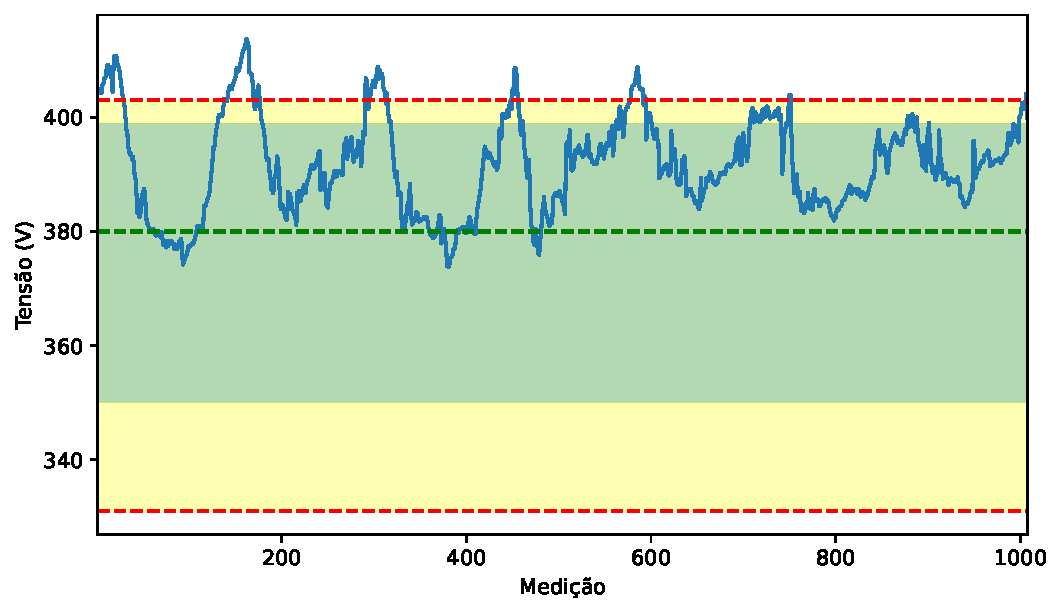
\includegraphics[width=16cm]{illustrations/figures/a1_V12_Max.pdf}
	\fonte{Autoria própria.}
\end{figure}

\begin{figure}[H]
	\centering
	\caption{Gráfico para tensão V23 de linha máxima}
    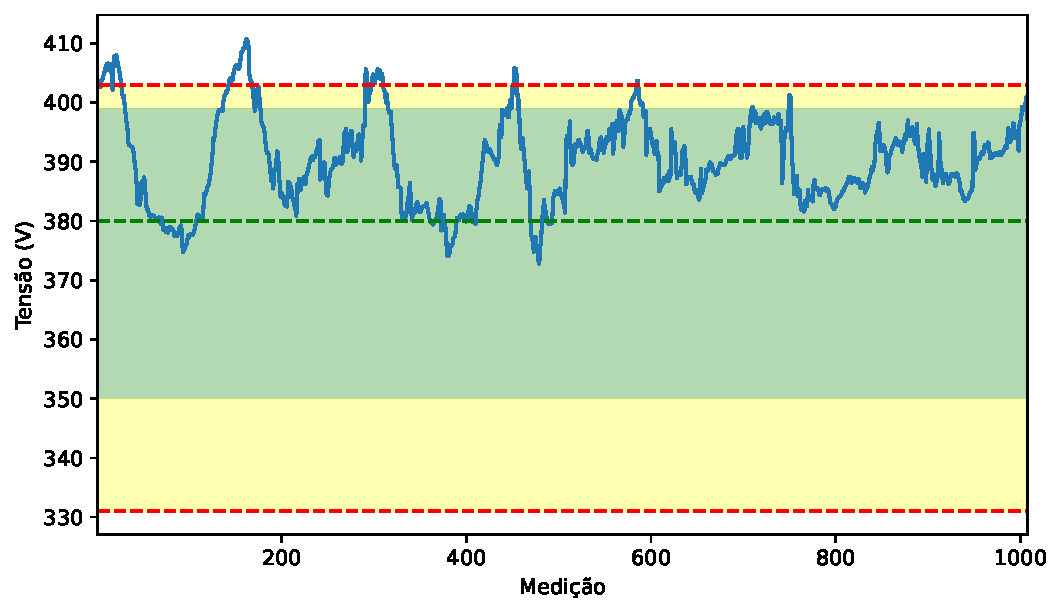
\includegraphics[width=16cm]{illustrations/figures/a1_V23_Max.pdf}
	\fonte{Autoria própria.}
\end{figure}

\begin{figure}[H]
	\centering
	\caption{Gráfico para tensão V31 de linha máxima}
    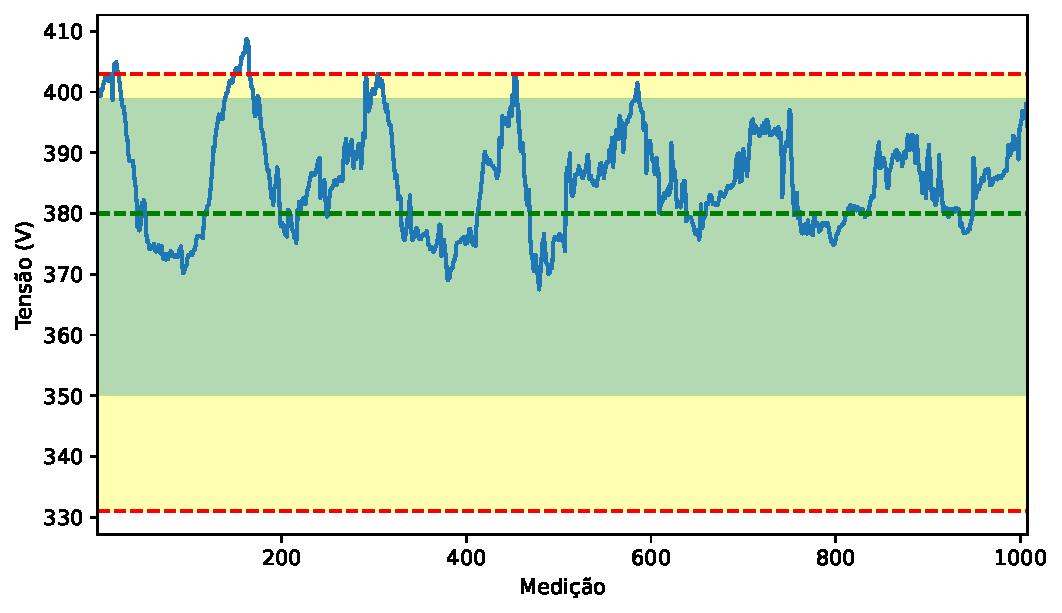
\includegraphics[width=16cm]{illustrations/figures/a1_V31_Max.pdf}
	\fonte{Autoria própria.}
\end{figure}

\begin{figure}[H]
	\centering
	\caption{Gráfico para tensão V12 de linha mínima}
    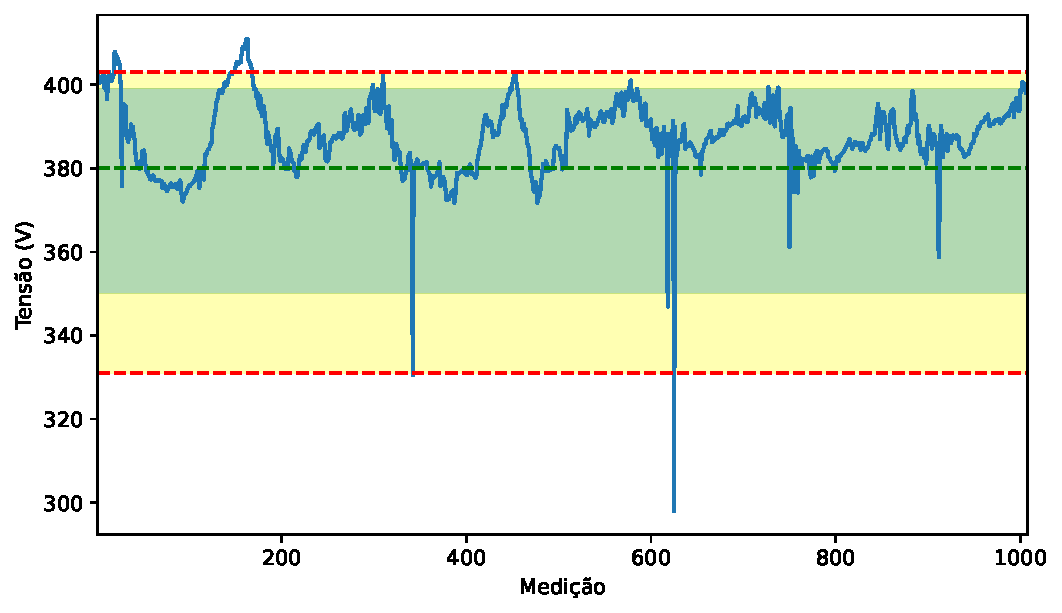
\includegraphics[width=16cm]{illustrations/figures/a1_V12_Min.pdf}
	\fonte{Autoria própria.}
\end{figure}

\begin{figure}[H]
	\centering
	\caption{Gráfico para tensão V23 de linha mínima}
    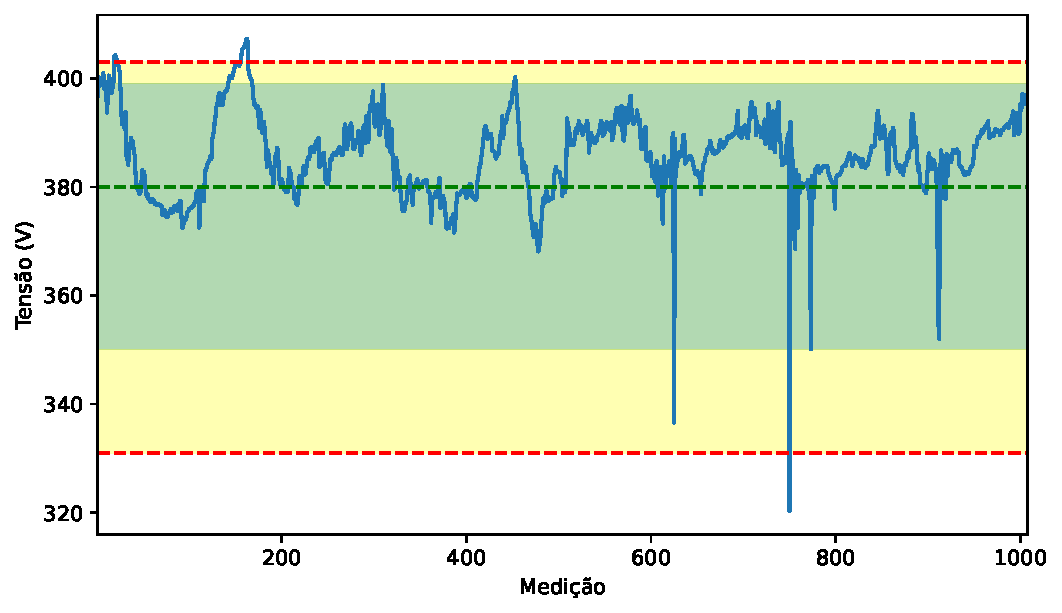
\includegraphics[width=16cm]{illustrations/figures/a1_V23_Min.pdf}
	\fonte{Autoria própria.}
\end{figure}

\begin{figure}[H]
	\centering
	\caption{Gráfico para tensão V31 de linha mínima}
    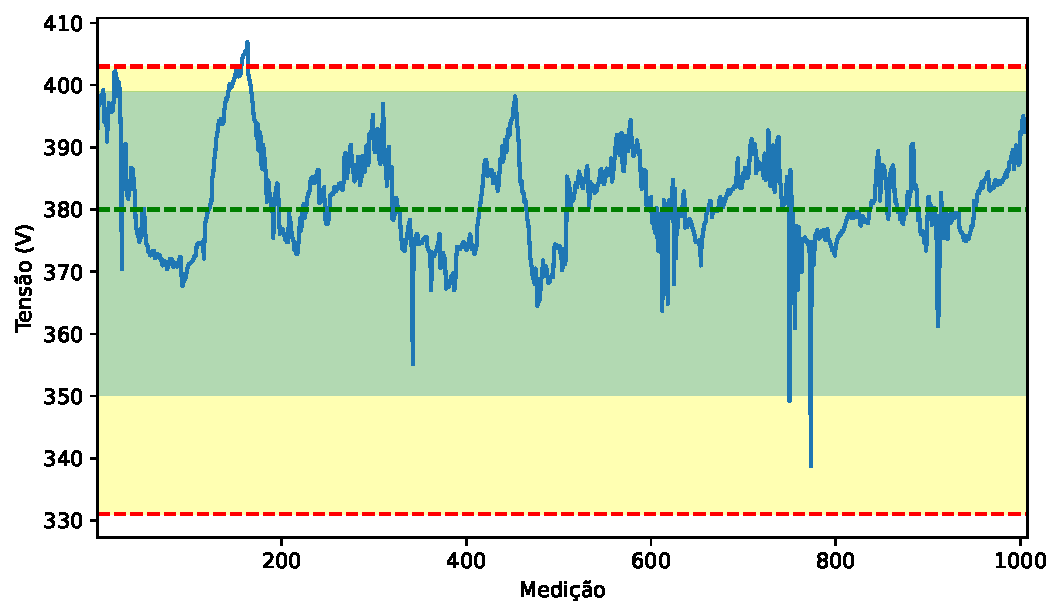
\includegraphics[width=16cm]{illustrations/figures/a1_V31_Min.pdf}
	\fonte{Autoria própria.}
\end{figure}

